\documentclass[12pt]{article}

\usepackage{sbc-template}

\usepackage{graphicx,url}
\usepackage{enumitem}
\usepackage{amsfonts}
\usepackage{verbatim}

\usepackage{booktabs}

\usepackage[brazil]{babel}   
%\usepackage[latin1]{inputenc}  
\usepackage[utf8]{inputenc}  
% UTF-8 encoding is recommended by ShareLaTex

     
\sloppy

\title{Padrões frequentes em comércio eletrônico}

\author{Raphael Correia de Souza Fialho\inst{1}}


\address{Programa de Pós-Graduação em Ciência da Computação -- CEFET/RJ\\
  CEP 20.271-110 -- Rio de Janeiro -- RJ -- Brasil
\email{raphael.fialho@b2wdigital.com}}


\begin{document} 

\maketitle

\begin{abstract}
   E-commerce websites use the A/B testing technique to decide how and what functionalities should be presented to end users, but this test does not identify the people profiles of who access the website, making it difficult to know the actual acceptance of the product for the desired audience.
   This research project proposes the development of an application that aims to categorize and distinguish the user profiles that access the website by machine learning methods using extracted frequency patterns. That way the business owner is be able to direct their e-commerce to the desired target audience without suffering distortions of the general appearance. The counselor pleaded is Prof. Dr. Eduardo Bezerra da Silva with coorientation of Prof. Dr. Eduardo Soares Ogasawara whose research project is Data and Application Management and the line of research is the Applications in Deep Learning and Pattern Recognition.
\end{abstract}
     
\begin{resumo} 
  Em websites de comércio eletrônico utiliza-se a técnica de teste A/B para decidir como e quais funcionalidades serão apresentadas aos usuários finais, porém este teste não identifica os tipos de pessoas que acessam o website, dificultando saber a real aceitação do produto para o público desejado.
  Este projeto de pesquisa propõe o desenvolvimento de uma aplicação que visa categorizar e distinguir os perfis de usuários que acessam o website usando métodos de aprendizado de máquina sob os padrões frequentes extraídos. Assim, o dono do negócio pode direcionar seu comércio eletrônico para o público-alvo desejado sem sofrer as distorções do aspecto geral. O orientador pleiteado é o Prof. Dr. Eduardo Bezerra da Silva com coorientação do Prof. Dr. Eduardo Soares Ogasawara cujo projeto de pesquisa é a Gerência de Dados e Aplicações e a linha de pesquisa é a Aplicações em Aprendizagem Profunda (Deep Learning) e Reconhecimento de Padrões.
\end{resumo}


\section{Introdução}

O Teste A/B é uma técnica de \textit{design} para decidir quais características causam maior aprovação dos usuários entre duas variantes: A e B. Duas versões de um mesmo \textit{website} são disponibilizados para seus usuários finais, onde para cada um é exibido apenas uma das versões, assim, é avaliado o grau de interesse e envolvimento de cada versão, medindo e avaliando a aceitação das funcionalidades.

A configuração experimental mais simples é avaliar um fator com dois níveis, um controle (versão A) e um tratamento (versão B). O controle é normalmente a versão padrão e o tratamento é a mudança que é testada. Essa configuração é comumente chamada de teste A/B. É comum ser estendido por vários níveis, muitas vezes referidos como testes de divisão A / B / N. Um experimento com
múltiplos fatores são referidos como \textit{Multivariable} (ou Multivariável) \cite{kohavi2010online}. A Figura \ref{fig:onlineExp1} demonstra a estrutura mais comum de um teste A/B.

\begin{figure}[ht]
\centering
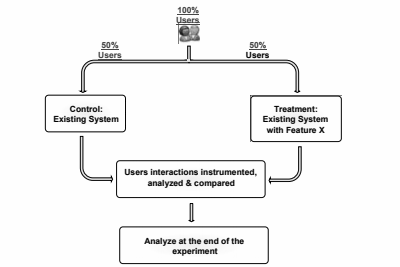
\includegraphics[width=.8\textwidth]{fig2.png}
\caption{Estrutura em alto nível de um experimento online. Usuários são divididos entre o sistema de controle e de tratamento. Interações dos usuários são instrumentadas, analisadas e comparadas. Análise no fim do experimento. Adaptado de \cite{kohavi2010online}.}
\label{fig:onlineExp1}
\end{figure}

O mapa \textit{heatmaps} destaca a influência do conteúdo da página onde as pessoas tendem a concentrar a visão, conforme a Figura \ref{fig:heatmap1}. Este é apenas alguns dos muitos métodos possíveis para entender as interações do usuário, e desenvolver hipóteses para testes controlados. Estudos de tração ocular mostram como as pessoas guiam sua atenção em uma página \cite{goward:13}.

\begin{figure}[ht]
\centering
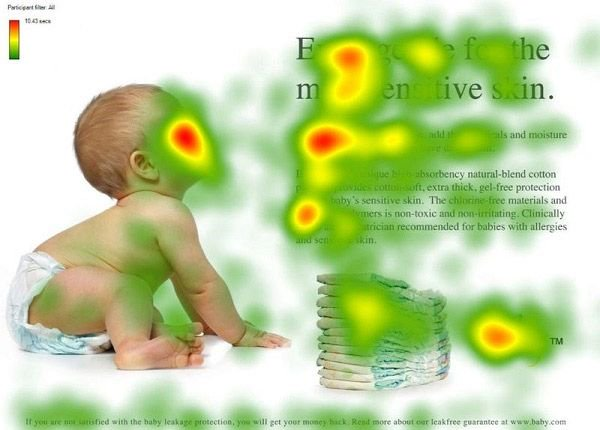
\includegraphics[width=.5\textwidth]{fig1.jpg}
\caption{Exemplo de heatmap. Áreas avermelhadas caracterizam zona de maior atenção pelos usuários. Adaptado de \cite{goward:13}.}
\label{fig:heatmap1}
\end{figure}

Através das informações do Teste A/B, mapa \textit{heatmaps} e outras provenientes dos dados de acesso capturados das entradas das requisições na página, como \textit{logs} das máquinas servidoras, podemos extrair, avaliar e categorizar automaticamente o perfil do usuário que acessa o \textit{website}.

Outras fontes de dados como a temperatura da cidade que o usuário está acessando, se está chovendo ou não, a hora do dia, a média da renda per capita da região, se há algum acontecimento relevante no dia como shows ou notícias, pode influenciar também no processo de categorização.

Após esta análise em \textit{BigData} de todas essas entradas, será possível identificar quais os perfis de usuários que mais estão sendo influenciados positivamente ou negativamente, para a dada hipótese testada sobre as funcionalidades incluídas no \textit{website}.

\section{Objetivos}
\subsection{Objetivo Geral}
Desenvolver uma aplicação para interpretar os resultados dos testes A/B, classificando os usuários pelas características dos dados durante o acesso, auxiliando, assim, o dono do negócio a direcionar sua marca a um ou mais públicos alvos.

\subsection{Objetivo Específico}
\begin{itemize}
\item Identificar os públicos de maior envolvimento e relevância;
\item identificando potenciais novos perfis que possam surgir ou desaparecer;
\item Sugerir opções que possam potencializar o envolvimento de um público.
\end{itemize}

\section{Método de Pesquisa}

A metodologia científica compreende basicamente um conjunto de dados iniciais e um sistema de operações ordenadas adequado para a formulação de conclusões, de acordo com certos objetivos predeterminantes \cite{tartuce:2006}.

Sendo assim, com o objetivo final da implementação da aplicação, esta se utilizará dos \textit{logs} de acesso dos servidores de aplicação, dados climáticos, geográficos e geopolíticos como conjunto de entrada de dados. Utilizará de recursos de aprendizagem de máquina para classificar e predizer os perfis de usuários derivados a partir dos padrões frequentes formados a partir da entrada.   

\section{Aprendizagem de máquina}

Em aprendizado de máquina, uma característica (em inglês, \textit{feature}) é uma propriedade mensurável de um fenômeno de interesse. Nesse contexto, são úteis transformações de uma representação de dados para outra em um nível conceitual mais alto e que possa ser efetivamente aproveitada por algoritmos de aprendizado. Tradicionalmente, algoritmos de aprendizado de máquina pressupõem que o conjunto de dados a ser usado no treinamento foi previamente construído por meio de um processo de engenharia de características \cite{bezerraintroduccao}.

As características dos usuários serão extraídos dos acessos captados pelo \textit{website} e captados de outras fontes externas, como temperatura local de onde partiu o acesso, índice de umidade relativa do ar, renda per capta da região, etc. Esses dados serão usados como fatores classificatórios para uma categoria de perfil de usuário durante o teste A/B. O intuito é que a aplicação desenvolvida seja capaz de aprender a identificar essas características observando o conjunto de funcionalidades testada no momento.

Será computado se as funcionalidades do sistema tratamento estão causando envolvimento positivo ou negativo para cada classe de usuários. Esse envolvimento será calculado de acordo com o tempo de permanência do usuário na página, número cliques gerados e clique no botão de fechamento de pedido.

\section{Resultados esperados}

\begin{itemize}[label={\checkmark}]
    \item Desenvolver a aplicação de forma plena e satisfatória;
    \item Sugerir melhorias (\textit{features}) que aumentem o envolvimento de um determinado perfil de usuário;
    \item Listar os públicos de maior envolvimento e relevância apontados por um determinado sistema tratamento;
    \item Listar novos perfis que se formam;
    \item Listar perfis que tendem a desaparecer;
    \item Publicação de experiências e pesquisas no âmbito acadêmico em forma de artigos, participação em congressos entre outros.
\end{itemize}

\bibliographystyle{sbc}
\bibliography{sbc-template}

\end{document}
